\usetikzlibrary{positioning}

\begin{document}

\def\title{Worksheet 3}

\newcommand{\qitem}{\qpart\item}

\renewcommand{\labelenumi}{(\alph{enumi})} % change default enum format to (a)
\renewcommand{\theenumi}{(\alph{enumi})} % fix reference format accordingly.
\renewcommand{\labelenumii}{\roman{enumii}.} % second level labels.
\renewcommand{\theenumii}{\roman{enumii}.}

\maketitle

\vspace{0.5em}

\begin{qunlist}

% Authors: Tony Li, and authors of diagonalization.tex
% Email: songli@berkeley.edu

\qns{Diagonalization and Diagonalizability}

\textbf{Diagonal matrices}, matrices where all entries outside of the diagonal are zero.
Diagonal matrices come handy in terms of solving systems of linear equations, solving for vector case of differential equations, finding out the determinant, etc. 
\newline \textbf{Diagonalization} is a procedure that we transform a matrix $A$ into three matrices multiplied together, whihc means 
$A=V{\Lambda}V^{-1}$, where $V^{-1}$ is the inverse of $V$, and $\Lambda$ is a diagonal matrix.

In this problem, we'll investigate what $V$ and $\Lambda$ truly are.

\begin{enumerate}

\qitem First we need to recall some pretty useful concepts, eigenvalues and eigenvectors. For a matrix $A$, if we can write the
equation that $A\vec{v}=\lambda\vec{v}$, where $\lambda$ is non-zero and $\vec{v}$ is non-zero vector, then we say that $\vec{v}$ and $\lambda$ is a pair of eigenvector and eigenvalue of $A$.
Given that 
$$A = \begin{bmatrix}
  2 & 2 \\
  5 & -1
  \end{bmatrix}$$
\textbf{Can you explain why $A$ has two eigenvalues and in a more general case, how many eigenvalues does a n by n matrix have?}
\ws{
\vspace{30px}
}

\meta{
  Introduce how we solve for eigenvalues and eigenvectors.
}

\sol{
  Based on the definition, we know $A\vec{v}=\lambda\vec{v}$, then we can write it into another form, $(A-{\lambda}I_n)\vec{v}=0$, where $I_n$
  is the identity matrix. As a result, since $\vec{v}$ can not be a zero vector, $(A-{\lambda}I_n)\vec{v}=0$ is a homogenous linear system solving for $\vec{v}$.
  $\vec{v}$ has non zero solution, only when $A-{\lambda}I_n$ is not invertible, which implies that $det(A-{\lambda}I_n)=0$.
  Solving a $det(A-{\lambda}I_n)=0$ is essentially solving a polynomial with degree n, so \textbf{$\lambda$ should have n solutions}.
  Plase note that, $\lambda$'s could be complex numbers.
}

\qitem \textbf{Find eigenvalues ${\lambda}_1$ and ${\lambda}_2$ and their corresponding eigenvectors $\vec{v_1}$ and $\vec{v_2}$}, where ${\lambda}_1\le{\lambda}_2$,
and both of the eigenvectors have length 1.

\ws{
\vspace{100px}
}

\sol{
  $$det(A-{\lambda}I_n)=det(\begin{bmatrix}
    2-\lambda & 2\\
    5 & -1-\lambda
  \end{bmatrix})=(2-\lambda)(-1-\lambda)-2\times5={\lambda}^2-\lambda-12=0$$
  \newline After solving the quadratic equation above, We have ${\lambda}_1=-3$ and ${\lambda}_2=4$.
  Let's plug two eigenvalues into $(A-{\lambda}I_n)\vec{v}=0$.
  $$\begin{bmatrix}
    2-{\lambda}_1 & 2\\
    5 & -1-{\lambda}_1 
  \end{bmatrix}\vec{v_1} = \begin{bmatrix}
    5 & 2\\
    5 & 2
  \end{bmatrix}\vec{v_1}=0$$
  $$\Rightarrow \vec{v_1}=\begin{bmatrix}
    2C\\
    -5C\\
  \end{bmatrix}, C\in\mathbb{R}$$
  Since $\vec{v_1}$ has length 1, then $$\vec{v_1}=\begin{bmatrix}
    \frac{2}{\sqrt{29}}\\
    \frac{-5}{\sqrt{29}}
  \end{bmatrix}$$
  \newline Similarly, we would have 
  $$\vec{v_2}=\begin{bmatrix}
    \frac{1}{\sqrt{2}}\\
    \frac{1}{\sqrt{2}}
  \end{bmatrix}$$
}

\end{enumerate}

With the eigenvectors $\vec{v_1}$ and $\vec{v_2}$, define $V$ to be the matrix:
$$V = \begin{bmatrix}
\vec{v_1} & \vec{v_2}
\end{bmatrix}$$
Columns of this matrix $V$ are called eigenbasis of $A$.
With the eigenvalues ${\lambda}_1$ and ${\lambda}_2$, define $\Lambda$ to be the matrix:
$$\Lambda = \begin{bmatrix}
  {\lambda}_1 & 0\\
  0 & {\lambda}_2
  \end{bmatrix}$$
\begin{enumerate}[resume]
\qitem Now, we need to \textbf{prove that $A=V{\Lambda}V^{-1}$}. Assume that $V$ is invertible.
\newline \emph{Hint:}First, transform the above equation into the form $AV=V{\Lambda}$. Then, expand $V$ and $\Lambda$ with
matrices provided above.
\ws{\vspace{100px}}

\meta{
  Show students that the procedure in the solution is applicable to prove $A=V{\Lambda}V^{-1}$, even if A is n by n.
}

\sol{
  Based on the definition of eigenvalues and eigenvectors, let $\vec{v_1}$, $\vec{v_2}$,..., $\vec{v_n}$ be n eigenvectors
  of the n by n matrix $A$, and their corresponding eigenvalues are ${\lambda}_1$, ${\lambda}_2$,..., ${\lambda}_n$.
  Now, we have $V=[\vec{v_1}, \vec{v_2}, ..., \vec{v_n}]$.
  $$AV=A[\vec{v_1}, \vec{v_2}, ..., \vec{v_n}]=[A\vec{v_1}, A\vec{v_2}, ..., A\vec{v_n}]=[{\lambda}_1\vec{v_1}, {\lambda}_2\vec{v_2}, ..., {\lambda}_n\vec{v_n}]$$
  $$=[\vec{v_1}, \vec{v_2}, ..., \vec{v_n}]\begin{bmatrix}
    {\lambda}_1&0&0&...\\
    0&{\lambda}_2&0&...\\
    ...&...&...&...\\
    0&0&...&{\lambda}_n
  \end{bmatrix}=V\Lambda$$
}
\qitem Now you know that in order to diagonalize a given matrix, we need to calculate eigenvalues and eigenvectors first. However, there is still a premise we need to deal with: \textbf{when is a matrix diagonalizable?
If a matrix is diagonalizable, does it imply that the matrix is also invertible? In the opposite direction, is an invertible matrix always diagonalizable?}
\ws{\vspace{40px}}

\meta{
  The essence of this question is to tell students that invertibility does not work here, and most students would tend to use invertibility
  to explain diagonalizability.
}

\sol {
  If we look at the steps of proving $A=V{\Lambda}V^{-1}$, we made assumption that proving $A=V{\Lambda}V^{-1}$ is equivalent to
  proving $AV=V\Lambda$. The only difference here is whether $V$, or the eigenbasis, is invertible. Therefore, if a matrix is diagonalizable,
  its eigenbasis should have n linearly independent eigenvectors, or the eigenbasis is invertible, or the determinant of eigenbasis is not 0.
  \newline The invertibility of the matrix itself does not imply its diagonalizability, and the diagonalizability also does not imply invertibility.
  \newline Counterexample of the first claim: 
  $$M=\begin{bmatrix}
    1&1\\
    0&1
  \end{bmatrix}$$
  Here, $M$ is invertible since $det(M)\ne0$, but it have two equal-value eigenvalues 1, which means that two eigenvectors can not be not
  linearly independent, so it is not diagonalizable.
  \newline Counterexample of the second claim:
  $$N=\begin{bmatrix}
    0&0\\
    0&1
  \end{bmatrix}$$
  In this case, $N$ is diagonalizable, since it has two distinct eigenvalues ${\lambda}_1=0$ and ${\lambda}_2=1$. Eigenvectors corresponding to distinct eigenvalues are linearly independent.
  However, $N$ is not invertible, because $det(N)=0$.
}
\end{enumerate}
Let's now concentrate on the diagonalization with help of change of basis. We'll explore the diagonalization more clearly from the
perspective of change of basis.
\begin{enumerate}[resume]

\qitem Let $\widetilde{\vec{x}}$ be the coordinates of $\vec{x}$ in the eigenbasis. 
This means that for some arbitrary vector represented in the eigenbasis $\widetilde{\vec{x}} = \begin{bmatrix} \alpha_1 \\ \alpha_2 \end{bmatrix}$, 
the corresponding representation in standard coordinates is a linear combination of the columns of $V$: $\vec{x} = \alpha_1 \vec{v_1} + \alpha_2 \vec{v_2}$. \textbf{What is $\widetilde{\vec{x}}$ in terms of $V$ and $\vec{x}?$}

(\textit{Hint: Write $\vec{x}$ in terms of $V$ and $\tilde{\vec{x}}$, then go from there.})

\ws{\vspace{3em}}

\meta{
  The line $\alpha_1 \vec{v_1} + \alpha_2 \vec{v_2} = V \widetilde{\vec{x}}$ is not the most intuitive.
  It may require you showing on the board, why matrix vector multiplication can be seen as a linear combination of the columns.
}

\sol{
  $\vec{x} = \alpha_1 \vec{v_1} + \alpha_2 \vec{v_2} = V \widetilde{\vec{x}}.$ So it follows that $\widetilde{\vec{x}} = V^{-1} \vec{x}.$
}

\qitem It is often helpful to visualize the change of basis in a state diagram, where \textit{each arrow represents left-multiplying the variable it's coming out of by the corresponding matrix.} \textbf{Fill in the missing matrix operations in the state diagram based on your answer from the previous part.}

\ws {
  \begin{figure}[H]
    \centering
    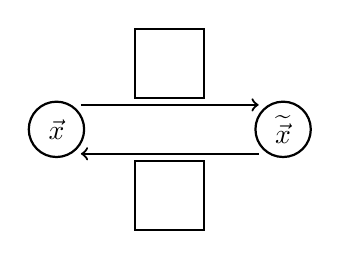
\begin{tikzpicture}[node distance = 2cm, thick,every node/.style={inner sep=0.25em,outer sep=0.25em}]%
      \node (1) [circle,draw,minimum size=2em] {$\vec{x}$};
      \node (2) [circle,draw,right=of 1,minimum size=2em] {$\widetilde{\vec{x}}$};
      \draw[->] (1.45) -- node [rectangle,draw,midway,above,minimum size=2.5em] {} (2.135);
      \draw[->] (2.225) -- node [rectangle,draw,midway,below,minimum size=2.5em] {} (1.315);
    \end{tikzpicture}%
  \end{figure}
}

\meta {
  Not everyone finds this diagram the most intuitive, but it definitely helps a large percentage of students. Stress to students that it's always better to understand the intuitive meaning behind change of basis than to remember any particular change of basis formula. This intuitive meaning is bridging between coordinate systems, which can be visualized with this diagram.
}

\sol {
  \begin{figure}[H]
  \centering
  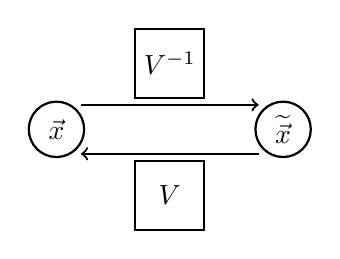
\begin{tikzpicture}[node distance = 2cm, thick,every node/.style={inner sep=0.25em,outer sep=0.25em}]%
    \node (1) [circle,draw,minimum size=2em] {$\vec{x}$};
    \node (2) [circle,draw,right=of 1,minimum size=2em] {$\widetilde{\vec{x}}$};
    \draw[->] (1.45) -- node [rectangle,draw,midway,above,minimum size=2.5em] {$V^{-1}$} (2.135);
    \draw[->] (2.225) -- node [rectangle,draw,midway,below,minimum size=2.5em] {$V$} (1.315);
  \end{tikzpicture}%
  \end{figure}
}


\qitem Now that we are able to switch back and forth between the coordinate systems, let's see how the linear transformation brought by $A$ can be viewed as a diagonal scaling transformation in the eigenbasis coordinate system.% Might be a bit confusing.

Let $\vec{y} = A \vec{x}$, and $\vec{x} = \alpha_1 \vec{v_1} + \alpha_2 \vec{v_2}$, using the same matrix $A$ and eigenvectors $\vec{v_1}, \vec{v_2}$ from before. Let $\widetilde{\vec{x}}$, $\widetilde{\vec{y}}$ be the coordinates of $\vec{x}$, $\vec{y}$ in the eigenbasis. \textbf{Find $\widetilde{\vec{x}}$ and $\widetilde{\vec{y}}$ in terms of $\alpha_1, \alpha_2, \lambda_1, \lambda_2$. What can we say about the relationship between $\widetilde{\vec{x}}$ and $\widetilde{\vec{y}}$?} % Might be confusing as to what the problem is asking compared to the next part.

(\textit{Hint}: Your answers shouldn't be in terms of the original $\vec{x}$ or $\vec{y}$.
 Use what you know about the coordinates of a vector in a certain basis; there is no need to invert any matrices or do any major computation.)

\ws {
  \vspace{200px}
}

\meta {
  Students may try to use what they found in the previous parts to multiply the vectors by $V^{-1}$. While this is technically right, make sure they understand what exactly
  that transformation is doing and why they don't need to do any matrix computation to find the coordinates of $\vec{y}$ in the eigenbasis.
}

\sol {
  $$\widetilde{\vec{x}} = \begin{bmatrix} \alpha_1 \\ \alpha_2 \end{bmatrix}$$

  \begin{align*}
    \vec{y} &= A \vec{x} \\
    &= A(\alpha_1 \vec{v_1} + \alpha_2 \vec{v_2}) \\
    &= \alpha_1 A \vec{v_1} + \alpha_2 A \vec{v_2} \\
    &= \alpha_1 \lambda_1 \vec{v_1} + \alpha_2 \lambda_2 \vec{v_2} \\
    \implies \widetilde{\vec{y}} &= \begin{bmatrix} \alpha_1 \lambda_1 \\ \alpha_2 \lambda_2 \end{bmatrix}
  \end{align*}

  This means that the matrix $D$ relating the two coordinates in the eigenbasis must be a diagonal scaling transformation, with the eigenvalues as the amount each dimension is scaled by.
}

\qitem \textbf{Find the matrix $D$ satisfying $\widetilde{\vec{y}} = D \widetilde{\vec{x}}$ in terms of $V$ and $A$.}

(\textit{Hint}: Start by writing $\vec{x}, \vec{y}$ in terms of $\widetilde{\vec{x}}$ and $\widetilde{\vec{y}}$. Refer to the state diagram from before.)

\ws{\vspace{240px}}

\meta {
  If students are comfortable with matrices representing linear transformations, you can explain this eigendecomposition as translating a linear transformation to and from the eigenbasis. For the diagonalization $A = VDV^{-1}$, left-multiplying an arbitrary vector $\vec{x}$ is equivalent to the following:

  \begin{align*}
    A \vec{x} &= VDV^{-1} \vec{x} \\
    &= VD \widetilde{\vec{x}} \\
    &= VD \begin{bmatrix} \alpha_1 \\ \alpha_2 \end{bmatrix} \\
    &= V \begin{bmatrix} \alpha_1 \lambda_1 \\ \alpha_2 \lambda_2 \end{bmatrix} \\
    &= V \widetilde{\vec{y}} \\
    &= \vec{y}
  \end{align*}
}

\sol {
  \begin{align*}
    \vec{y} &= A \vec{x} \\
    V \widetilde{\vec{y}} &= A V \widetilde{\vec{x}} \\
    \widetilde{\vec{y}} &= V^{-1} A V \widetilde{\vec{x}} \\
    \implies D &= V^{-1} A V
  \end{align*}
}

\qitem Finally, let's visualize this linear transformation $A$ from the perspective of two different coordinate systems in the state diagram below. \textbf{Fill in the missing matrix operations in the state diagram. How can you show and explain the diagonalization $A = VDV^{-1}$ (using the state diagram) and the change of basis perspective?}

\ws {
  \begin{figure}[H]
    \centering
    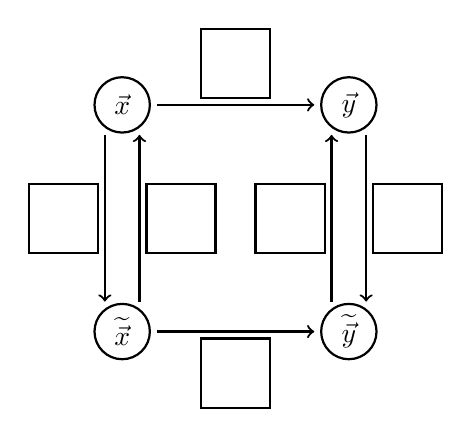
\begin{tikzpicture}[node distance = 2cm, thick, every node/.style={inner sep=0.25em,outer sep=0.25em}]%
      \node (1) [circle,draw,minimum size=2em] {$\vec{x}$};
      \node (2) [circle,draw,right=of 1,minimum size=2em] {$\vec{y}$};
      \node (3) [circle,draw,below=of 2,minimum size=2em] {$\widetilde{\vec{y}}$};
      \node (4) [circle,draw,below=of 1,minimum size=2em] {$\widetilde{\vec{x}}$};
      \draw[->] (1) -- node [rectangle,draw,midway,above,minimum size=2.5em] {} (2);
      \draw[->] (1.240) -- node [rectangle,draw,midway,left,minimum size=2.5em]{} (4.120);
      \draw[->] (4.60) -- node [rectangle,draw,midway,right,minimum size=2.5em]{} (1.300);
      \draw[->] (2.300) -- node [rectangle,draw,midway,right,minimum size=2.5em]{} (3.60);
      \draw[->] (3.120) -- node [rectangle,draw,midway,left,minimum size=2.5em]{} (2.240);
      \draw[->] (4) -- node [rectangle,draw,midway,below,minimum size=2.5em] {} (3);
    \end{tikzpicture}%
  \end{figure}
}

\sol {
  \begin{figure}[H]
    \centering
    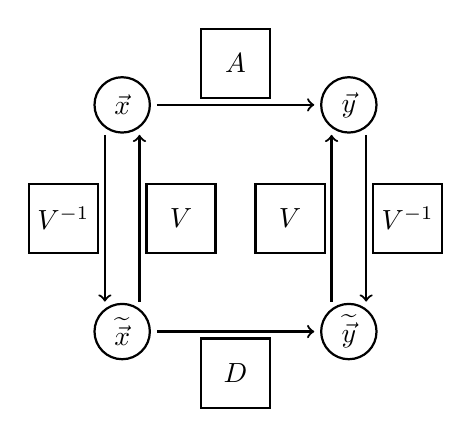
\begin{tikzpicture}[node distance = 2cm, thick, every node/.style={inner sep=0.25em,outer sep=0.25em}]%
      \node (1) [circle,draw,minimum size=2em] {$\vec{x}$};
      \node (2) [circle,draw,right=of 1,minimum size=2em] {$\vec{y}$};
      \node (3) [circle,draw,below=of 2,minimum size=2em] {$\widetilde{\vec{y}}$};
      \node (4) [circle,draw,below=of 1,minimum size=2em] {$\widetilde{\vec{x}}$};
      \draw[->] (1) -- node [rectangle,draw,midway,above,minimum size=2.5em] {$A$} (2);
      \draw[->] (1.240) -- node [rectangle,draw,midway,left,minimum size=2.5em]{$V^{-1}$} (4.120);
      \draw[->] (4.60) -- node [rectangle,draw,midway,right,minimum size=2.5em]{$V$} (1.300);
      \draw[->] (2.300) -- node [rectangle,draw,midway,right,minimum size=2.5em]{$V^{-1}$} (3.60);
      \draw[->] (3.120) -- node [rectangle,draw,midway,left,minimum size=2.5em]{$V$} (2.240);
      \draw[->] (4) -- node [rectangle,draw,midway,below,minimum size=2.5em] {$D$} (3);
    \end{tikzpicture}%
  \end{figure}

  You can explain $A = VDV^{-1}$ by just left-multiplying in the order of the arrows from $\vec{x}$ to $\vec{y}$. Again, in the change of basis perspective, $V^{-1}$ first pulls the vector $\vec{x}$ into the eigenbasis. $D$ performs the equivalent linear transformation of $A$ but in the eigen-coordinate system. Finally, $V$ brings the transformed vector back into standard coordinates.
}

\end{enumerate}

\newpage
\input{\bank/vector-diff-eq/vector_diff_eq}
\newpage
\input{\bank/phasors/phasors_intro}
\end{qunlist}

\end{document}
